\documentclass[10pt,a4paper]{article}
% ========================== DO NOT MODIFY =================================== %
\usepackage[a4paper,left=2.0cm,top=2.0cm,right=2.0cm,bottom=2.0cm]{geometry}
\usepackage{amssymb,amsmath} % If amsmath is required
\usepackage{url}
\usepackage{times}
\usepackage{mathptmx}      %% use fitting times fonts also in formulas
\usepackage{graphicx}
\usepackage{titling}
\usepackage{authblk}
\usepackage{multicol}
\usepackage{float}
\usepackage{enumitem}
\usepackage[small,compact]{titlesec}
\usepackage[numbers,sort&compress]{natbib}
\usepackage[T1]{fontenc}
\usepackage[UKenglish]{babel}
\usepackage[small,bf,tableposition=top,figureposition=bottom,skip=2pt]{caption}
\usepackage{subcaption}
\usepackage{booktabs}


% limit space between floats and text
\setlength{\textfloatsep}{10pt plus 1.0pt minus 2.0pt}
% shrink the list environments
\setlist{noitemsep}
\setlist{nolistsep}

% Shrink the bibliography
  \let\oldthebibliography=\thebibliography
  \let\endoldthebibliography=\endthebibliography
  \renewenvironment{thebibliography}[1]{%
    \begin{oldthebibliography}{#1}%
      \setlength{\parskip}{0ex}%
      \setlength{\itemsep}{0ex}%
  }%
  {%
    \end{oldthebibliography}%
  }

% Format of the front matter
\renewcommand{\Affilfont}{\small}
\setlength{\affilsep}{1ex}
\renewcommand\Authands{, }
\setlength{\droptitle}{-1.634cm}
% ============================================================================ %


% To be able to type european characters without escape sequences
% uncomment according to your operating system, if desired:
% ---------------------------------------------------------------------------- %
% \usepackage[latin1]{inputenc}   %% (Windows, old Linux)
% \usepackage[utf8]{inputenc}     %% (Linux)
% \usepackage[applemac]{inputenc} %% (Mac OS)
% ---------------------------------------------------------------------------- %


%------------------------------- FRONT MATTER -------------------------------- %
\title{EIDORS Version 3.8%
\vspace{-2ex}} %remove vertical space
\author[1]{Andy~Adler}
\author[1]{Alistair~Boyle}
\author[2]{Michael~G.~Crabb}
\author[1]{Herv{\'e}~Gagnon}
\author[3]{Bart{\l}omiej~Grychtol}
\author[4]{Nolwenn~Lesparre}
\author[2]{William~R.~B.~Lionheart}
\affil[1]{Carleton University, Ottawa, Canada}
\affil[2]{University of Manchester, Manchester, UK}
\affil[3]{Fraunhofer Project Group for Automation in Medicine and Biotechnology PAMB, Mannheim, Germany}
\affil[4]{IRSN, B.P. 17, 92262 Fontenay-aux-Roses Cedex, France.}
\date{}
%----------------------------------------------------------------------------- %



\begin{document}
\maketitle
\vspace{-1.5cm}
\thispagestyle{empty}

\begin{multicols}{2}

\noindent {\bf Abstract:} %The abstract should contain no more than 8
%lines of text and describe the main methods and findings.
This paper announces the release of version 3.8 of the
EIDORS software suite. We review its new features, and 
discusses recent successes and challenges.

\section{Introduction}
We are pleased to announce the release of EIDORS~3.8 (fig.~\ref{fig:logo}).
The software is available at \url{www.eidors.org} and is licensed under the GNU GPLv2.

EIDORS aims to provide free software algorithms for forward modelling
and inverse solutions
of Electrical Impedance and (to some extent) Diffusion-based Optical Tomography, in
medical, industrial and geophysical settings and to share data and promote
collaboration.

\begin{figure}[H]
  \vspace{-4.5mm}
\centering
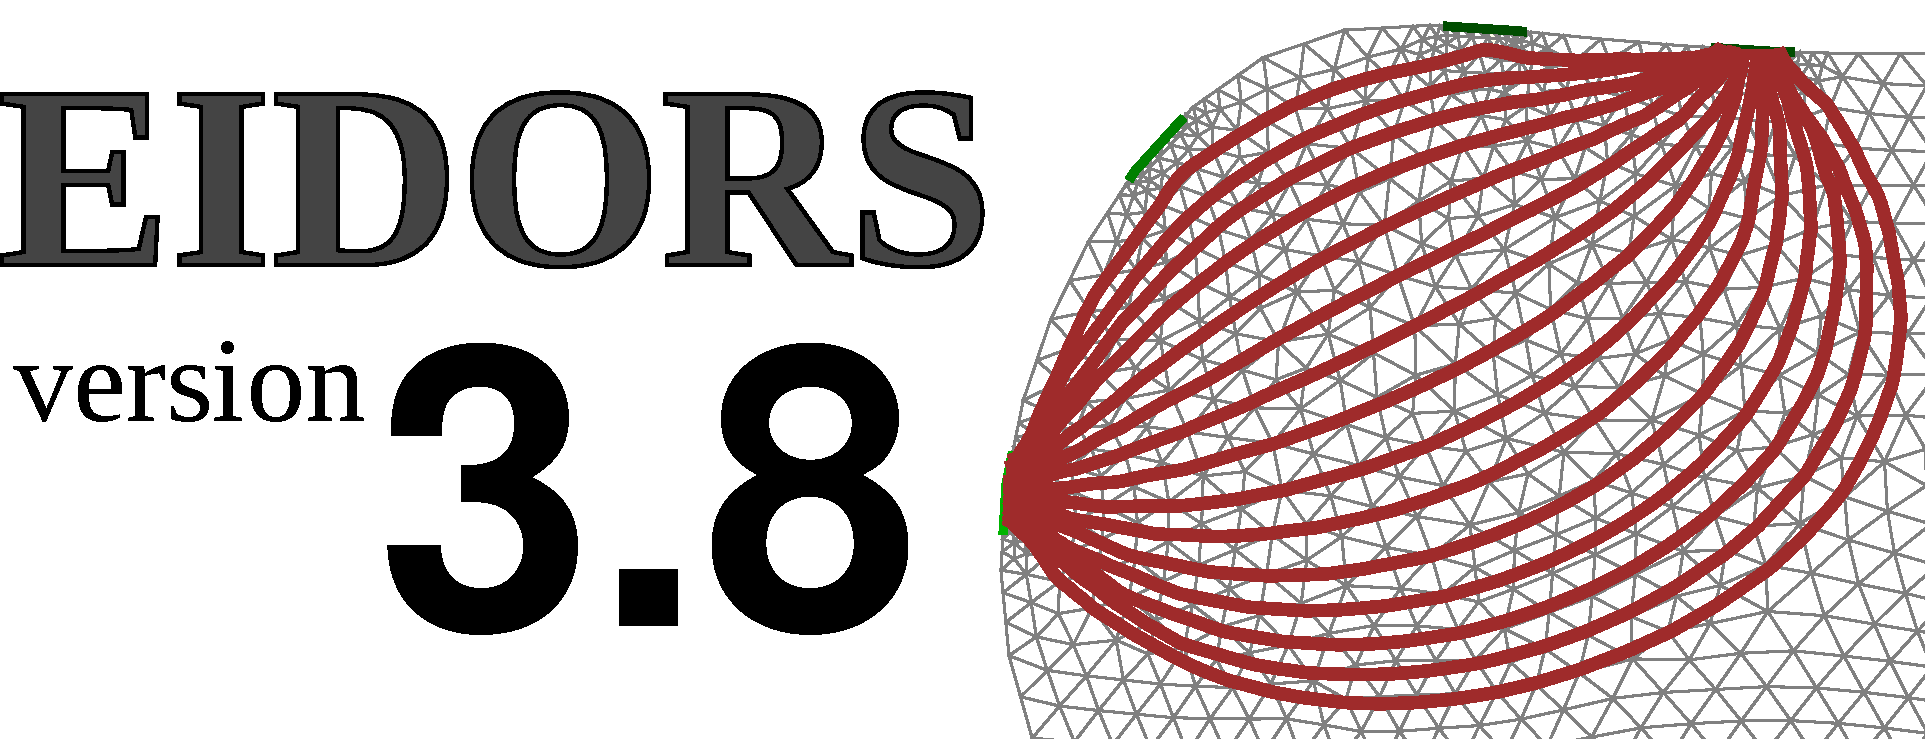
\includegraphics[width=.75\columnwidth]{mesh-eidors3p8.pdf}
\caption{\label{fig:logo}%
  EIDORS 3.8: featuring flexible parametrization, meshing, absolute solver and visualization improvements.
  Image shows current streamlines on a thorax-shaped finite element model.
%  Blobby the Walrus is pleased to announce...\\
%  \footnotesize Derived: ``Walrus hunk'' by claumoho (flickr.com) / CC BY 2.0 Attribution
}
\end{figure}
\vspace{-1.5em}

\section{New Features}
Release 3.8 of EIDORS builds upon a strong foundation in reconstruction
algorithms, adding and improving a number of aspects.
\begin{enumerate}
\item More stable
  iterative absolute inverse solvers (both Gauss-Newton and
  Conjugate-Gradient).
% DEPENDS ON ABS SOLVER

\item Greater flexibility in parametrization choices.
% DEPENDS ON ABS SOLVER

\item Native handling of unit scaling ($10^x$, $e^x$, $\ln x$, $\log_{10} x$),
 and arbitrary units.
% resistivity/conductivity, and apparent resistivity conversions.
  Natural limits for $\sigma > 0$. %~\cite{polydorides2014}.
% A framework for alternate arbitrary units.
%  Support for transparent usage in forward solutions and
%  Jacobian calculations.
% DEPENDS ON ABS SOLVER

\item GREIT reconstructions in 3D

\item Speed optimizations: improved Jacobian calculation, faster cache handling, and 
% Improvements to {\tt stim\_meas\_list} generated structures, resulting in
  faster forward solutions.
%  Also, the ability to
%  convert between a stimulus structure and a list of stimulus and measurement electrode pairs.
% An implementation of the parallel Jacobian calculator (pending MEX issues).

%\item Attempts to work around broken matlab MEX file handling (cross-platform mex compile).

\item Improved interfaces to NetGen and visualization.
      Compound and point electrodes in NetGen.

\item Analytic calculation of dual-mesh interpolations (coarse to fine)
% as well as, Quad and hex shaped mesh elements %rev 4392

\item Support for second and third order mesh elements.

\item Support for Dr\"ager and Swisstom file formats
%\item OpenEIT file format support~\cite{jones2014}.

\item Expanded shape library
\end{enumerate}

\section{Growth}
EIDORS-related citations continue to grow. Current citation results are
shown in table~\ref{tbl:cite}.

The EIDORS code-base is stable with significant effort being applied to
improving test coverage, refining performance and implementing new features
(fig.~\ref{fig:loc}).

\begin{figure}[H]
  \vspace{-2.5mm}
\centering
% trim=left botm right top
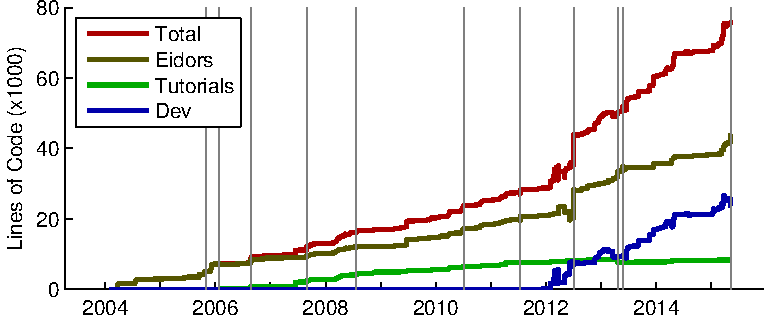
\includegraphics[width=.96\columnwidth]{fig_loc.pdf}
\caption{\label{fig:loc}%
%graph and table combo chart, including line for test code.
  Lines of Code (LoC) in Matlab files in the EIDORS code-base vs.\ time; Total
   (red), Eidors (i.e.\ release branch, yellow), Tutorials (green), development code (blue).
   Releases are indicated by gray bars.
}
\end{figure}
\vspace{-1.5em}
\begin{table}[H]
  \footnotesize
\centering
%From: http://amath.colorado.edu/documentation/LaTeX/reference/tables/ex1.html
\caption{\label{tbl:cite} EIDORS Citations
 (May 2014, scholar.google.com).
}
\begin{tabular}{lr}
  \toprule
  Paper & Citations \\
  %{@{\extracolsep{\fill}}@{}|c|ccc|r|}
  \midrule
  \cite{vauhkonen2001} A MATLAB package for the EIDORS project {\tiny ...}  & 159 \\
  \cite{polydorides2002phd} Image reconstruction algorithms for {\tiny ...}  & 88 \\
  \cite{polydorides2002matlab} A Matlab toolkit for three-dimensional {\tiny ...}  & 293 \\
  \cite{adler2006} Uses and abuses of {EIDORS}: An extensible {\tiny ...} & 184 \\
  \bottomrule
\end{tabular}
\vspace{-1em}
\end{table}

\section{Successes}
The structure of EIDORS has been relatively stable due, in part, to some early design choices:
a modular framework and data structure,
cross-platform support, integration of meshing,
tutorials, and the contributed data repository.
These aspects, along with an open source code-base, have enabled EIDORS to
maintain research relevance.

\section{Challenges}
A number of challenges inherent in the implementation of EIDORS as a Matlab-based toolkit continue to recur.
There is no real Object Oriented framework: no reflection, protection, or
  automatic management of errors.
Versions of Matlab frequently vary in confounding ways that make
  maintaining a toolkit across multiple Matlab versions difficult. This is
  particularly prevalent for Windows users and ``mex" file compilation.
The data structure and subfunction complexity in EIDORS are a
  source of confusion for beginners.
% and a challenge to manage for developers.
%The expansion of EIDORS into new application domains continues to provide software development challenges at times.
%Despite this, or indeed because of this, 
Despite these challenges, EIDORS continues to develop and grow at a healthy pace.

In short, EIDORS version 3.8 represents the continued development
in a healthy open-source software project.

\section*{Acknowledgements}
Recent funding for EIDORS development thanks to
Swisstom AG, NSERC Canada, and EPSRC UK.

\footnotesize
\begin{thebibliography}{}
%\bibitem{polydorides2014}
%Polydorides N, Ouypornkochagorn T, McCann H. 
%{\em Proc 15th Conf}, EIT, Gananoque, Canada, 2014
\bibitem{vauhkonen2001}
   Vauhkonen M, Lionheart WRB, Heikkinen L, et al
   {\em  Physiol Meas} 22:107--111, 2001
\bibitem{polydorides2002phd}
   Polydorides N.
 {\em Image Reconstruction Algorithms for Soft-Field Tomography}, Ph.D. thesis, University of Manchester, UK, 2002
\bibitem{polydorides2002matlab}
   Polydorides N, Lionheart WRB.
   {\em Meas Sci and Tech} 13:1871--1883, 2002
\bibitem{adler2006}
Adler A, Lionheart WRB. {\em Physiol Meas} 27:S25--S42, 2006
\end{thebibliography}
\end{multicols}

\end{document}
